\documentclass[12pt, a4paper]{article}

\usepackage[utf8]{inputenc}
\usepackage{lmodern}
%\usepackage{fourier}
\usepackage{setspace}
	\singlespacing

\usepackage[frenchb]{babel}
\usepackage{xspace}
\usepackage[margin= 2.5cm]{geometry}
\pagestyle{plain}
\renewcommand{\thefootnote}{\fnsymbol{footnote}}

\usepackage{tikz}
	\usetikzlibrary{shapes}
\usepackage{graphicx}
	\graphicspath{{img/}}

\usepackage{varioref}
	\renewcommand{\reftextbefore}{page précédente}
	\renewcommand{\reftextfacebefore}{page ci-contre}
	\renewcommand{\reftextafter}{page suivante}
	\renewcommand{\reftextfaceafter}{page ci-contre}
	\renewcommand{\reftextcurrent}{}

\usepackage{amsmath, amsfonts}
\everymath{\displaystyle}


\newcommand{\espace}{\vspace{.8cm}}
\newcommand{\pg}{

}

%% REMPLIR
\usepackage[colorlinks=true, allcolors=blue, pdfborder={0 0 0}]{hyperref}
	\hypersetup{
		pdftitle={Super Twitter},
		pdfsubject={Rapport Super Twitter},
		pdfkeywords={Suter Twitter, IARISS, raport},
		pdfauthor={IARISS Team}
	}
\title{Défi Super Twitter}
\newcommand{\authors}{Florent}

%
\begin{document}

\author{
\includegraphics{../_img/iariss_team.png} \\ {\sffamily \href{http://iarissteam.me}{iarissteam.me}}}
\date{\today}

\maketitle{}

{\sffamily Ce rapport a pour but de montrer quels ont été les méthodes et les moyens mis en place pour assurer une présence intensive sur les réseaux sociaux, notamment Twitter, tout au long de la \#nuitinfo !} 

\espace{}
Bien avant le début de la nuit, nous avons commencé à assurer une présence soutenue sur Twitter. Le jour J, notre présence a été encore plus importante : nous avons attend la limite fixée pour Twitter, à savoir 1000 tweets par jour ! Ce qui nous a vallu d'être bloqué durant quelques heures, et nous a obligé à créer un autre compte, \@TheIariss Team, afin de pouvoir continuer à Twitter sur la Nuit de l'Info.

Afin de s'assurer une bonne visibilité, chaque membre de l'équipe s'est créé un compte Twitter, afin de pouvoir tweeter sur la nuit de l'info, et re-tweeter certains tweets. L'équipe avait également un compte Twitter au nom de l'équipe, à savoir \@IarissTeam.

Nous avons eu, durant toute la soirée, une équipe dont le but quasi-exclusif était d'envoyer et de répondre aux tweets.

Nous avons également utilisé le logiciel TweetDeck, afin de nous faciliter la tâche et de pouvoir assurer un bon suivi de nos tweets : 

\espace{}
\begin{center}
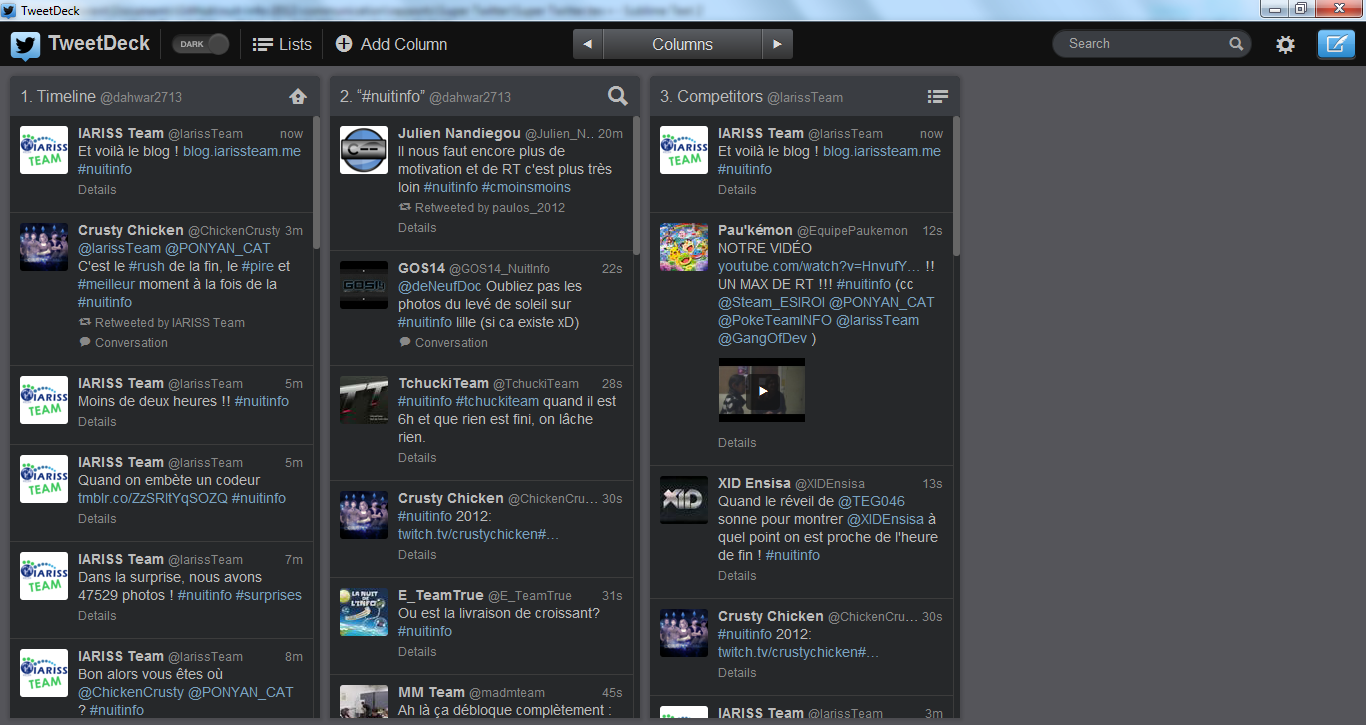
\includegraphics[width=.9\textwidth, keepaspectratio=true]{img/tweetdeck.png}
\end{center}
\espace{}

Pour conclure, nous pouvons dire que les tweets se sont enchainés à un rythme effréné toute la soirée, mais nous pensons avoir quand même réussi à assurer une bonne présence.


%\espace{}
%\begin{figure}[h]
%	\begin{center}
%	\end{center}
%	\caption{\label{fig-} Légende}
%\end{figure}

\espace\vfill{}
Ce document a été rédigé en \LaTeX{} par \authors{} pour IarissTeam avec quelques tasses de café et beaucoup de bonne humeur.

Contactez-nous à \href{mailto:nuitinfo@iariss.com}{nuitinfo@iariss.com} pour tout renseignement supplémentaire !

\end{document}